\textbf{Входные параметры:}
 
 Parent1 --- первый родитель;
 
 Parent2 --- второй родитель;
 
 VHML\_ResultVector --- потомок;
 
 VHML\_N --- размер векторов Parent1, Parent2 и VHML\_ResultVector.

\textbf{Возвращаемое значение:}

 Отсутствует.
 
\textbf{ Примечание:}

 Потомок выбирается случайно.
 
\begin{align}
&Crossover \left( \overline{Parent}^1, \overline{Parent}^2, DataOfCros\right)=Random \left(\left\lbrace \overline{Offspring}^1; \overline{Offspring}^2\right\rbrace  \right),\nonumber \\
&r_1=Random\left( \left\lbrace 2; 3; \ldots; n\right\rbrace \right); \nonumber \\
&r_2=Random\left( \left\lbrace 2; 3; \ldots; n\right\rbrace \right); \nonumber \\
&R_1=\min \left( r_1, r_2\right) ; \nonumber \\
&R_2=\max \left( r_1, r_2\right) ; \nonumber \\
& \overline{Offspring}^1_i=\overline{Parent}^1_i, i=\overline{1,R_1-1};\nonumber\\
& \overline{Offspring}^1_i=\overline{Parent}^2_i, i=\overline{R_1,R_2-1};\nonumber\\
&  \overline{Offspring}^1_i=\overline{Parent}^1_i, i=\overline{R_2,n};\nonumber\\
& \overline{Offspring}^2_i=\overline{Parent}^2_i, i=\overline{1,R_1-1};\nonumber\\
& \overline{Offspring}^2_i=\overline{Parent}^1_i, i=\overline{R_1,R_2-1};\nonumber\\
&  \overline{Offspring}^2_i=\overline{Parent}^2_i, i=\overline{R_2,n};\nonumber\\
&\overline{Offspring}^1\in X, \overline{Offspring}^2\in X.
\end{align}

$ DataOfCros $ не содержит каких-либо параметров относительно данного типа скрещивания.

\textbf{Пример.} Двухточечное скрещивание показано на рисунке:

\begin{figure} [h]
  \center
  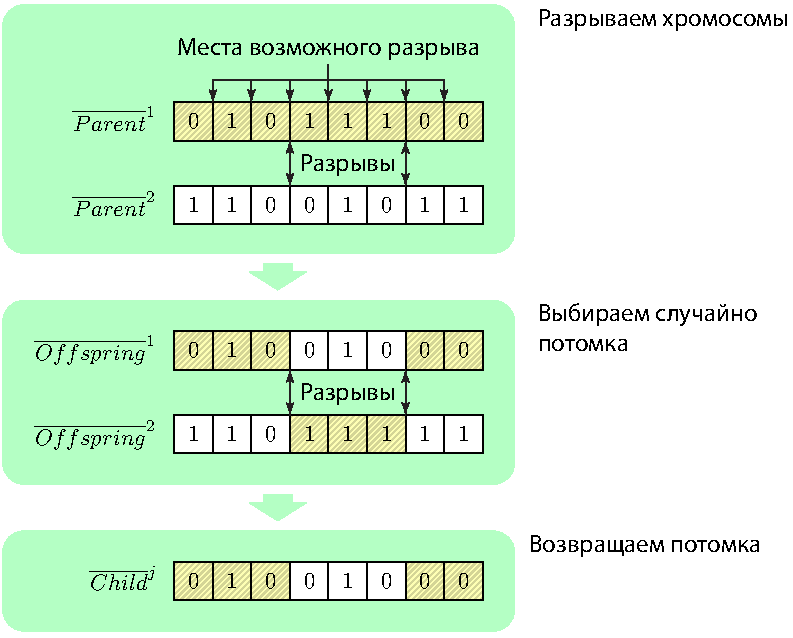
\includegraphics [scale=0.8] {HML_TwopointCrossover_Sheme}
  \caption{Механизм работы двухточечного скрещивания} 
  \label{img:HML_TwopointCrossover_Sheme}  
\end{figure}